% 下面方法是 vlm-based 的人形vla的文章
% https://arxiv.org/pdf/2603.12263
% https://arxiv.org/pdf/2607.18016
% https://arxiv.org/pdf/2503.14734
% https://arxiv.org/pdf/2608.16837
% https://arxiv.org/pdf/2510.03022
% https://arxiv.org/pdf/2606.22174
% https://arxiv.org/pdf/2603.05410
% https://arxiv.org/pdf/2603.09170v1

% 下面方法是 vgm-based 的人形vla 的文章
% https://arxiv.org/pdf/2608.06375
% https://arxiv.org/pdf/2606.09215
% https://arxiv.org/pdf/2609.16644v1

% Local spacing keeps the Introduction and contributions together.
\begingroup
\linespread{0.97}\selectfont
\setlength{\parskip}{0.25em plus 0.05em minus 0.03em}
\setlength{\textfloatsep}{10pt plus 2pt minus 2pt}
\suppressfloats[t]
\begin{figure*}[t]
  \centering
  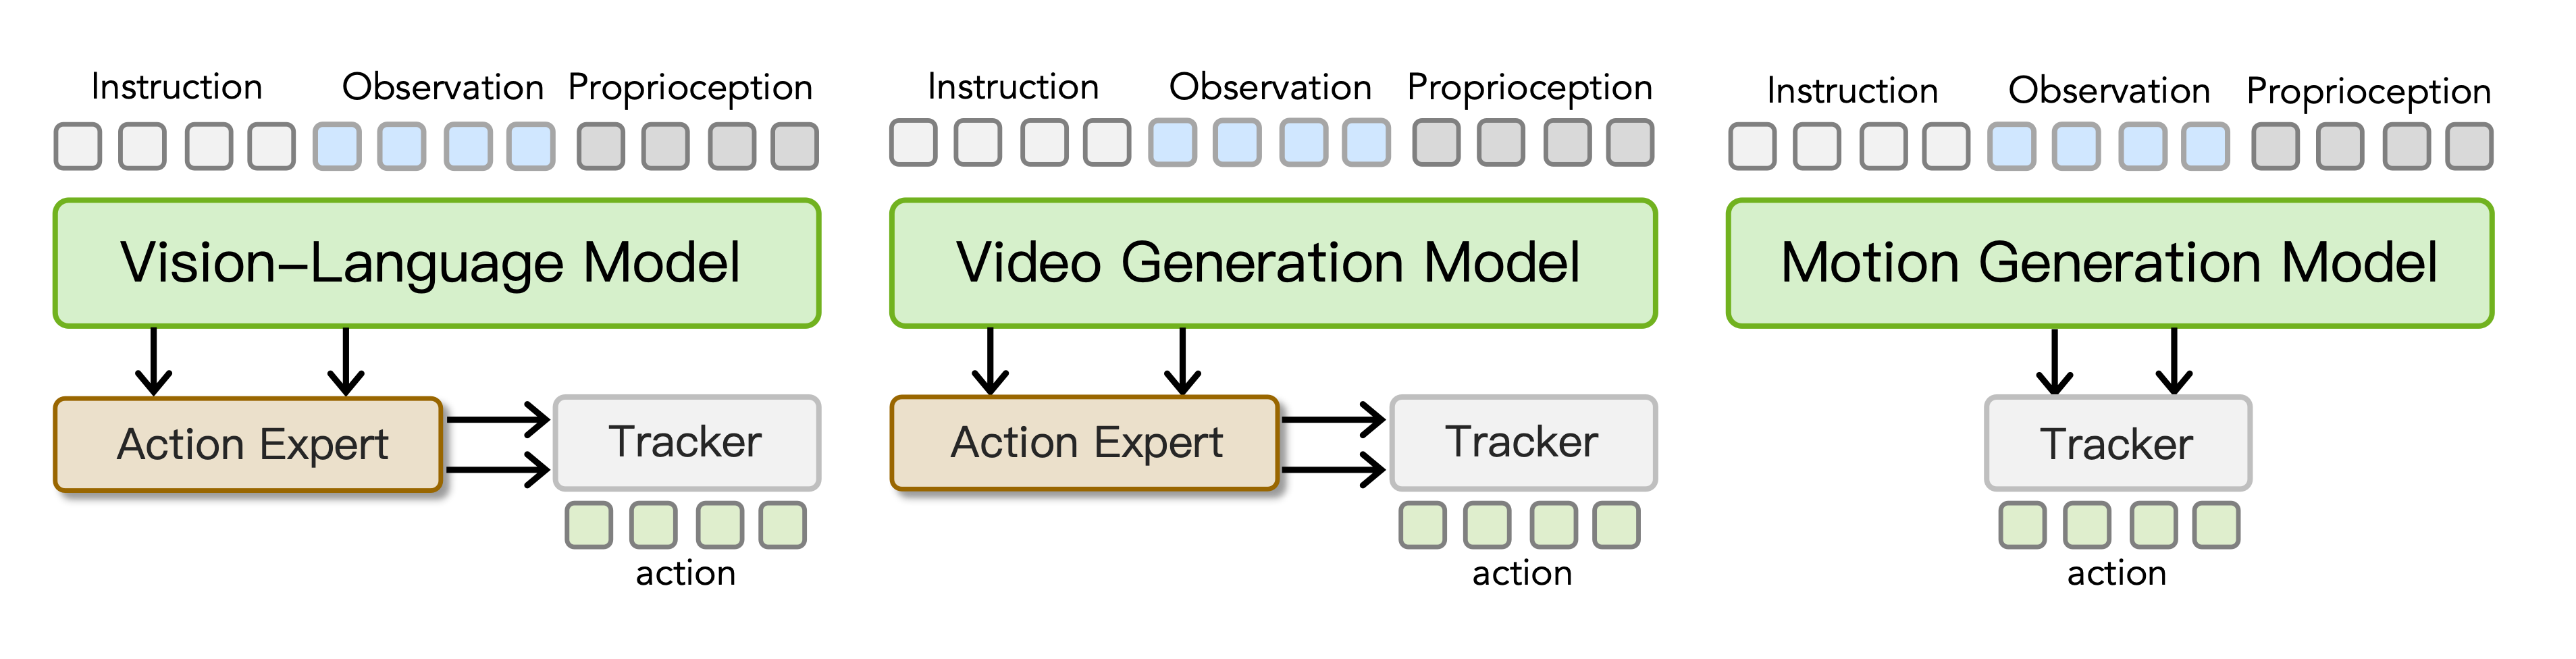
\includegraphics[width=0.98\textwidth]{image/intro.png}
  \caption{\textbf{Pretrained Backbones for Humanoid Action Generation.}
  From left to right: VLA, WAM, and KAM paradigms built around vision--language, video generation, and motion generation models.
  The schematic highlights their primary sources of generative priors: KAMs adapt a pretrained motion generator to produce kinematic action sequences for a downstream tracker, directly transferring learned movement structure into the policy.}
  \label{fig:policy_routes}
\end{figure*}

Humanoid loco-manipulation integrates task understanding, visual perception, and high-dimensional whole-body coordination~\citep{psi0,openhlm}. Beyond the requirements of conventional manipulation, it demands that robots continuously coordinate their root, torso, arms, and legs throughout an interaction~\citep{leverb}. For example, reaching for an object while moving requires a robot to simultaneously adjust its body position, maintain dynamic balance, and coordinate joint movements according to the object's location and contact state. Whole-body motion is therefore an integral part of accomplishing the task, rather than merely an execution stage that follows task-level decision-making. Even with accurate task understanding and perception, a robot cannot complete the task without generating temporally and spatially coordinated, executable whole-body motion. The central challenge of loco-manipulation thus extends beyond determining what the robot should do to generating the high-dimensional, continuous, and coupled whole-body motion required for task execution.

Recent advances in vision--language--action models (VLAs) and world action models (WAMs) offer two representative approaches to robot action generation. VLAs typically extend the semantic understanding and visual representations acquired by pretrained vision--language models to robot action prediction~\citep{rt2,openvla,pi0,grootn1}. WAMs draw on the visual dynamics learned by pretrained video generation models to connect future-state prediction with action generation~\citep{dreamzero,motionwam,wholebodywam_wbc}. These approaches provide important foundations for task understanding, environmental perception, and interaction planning. However, pretrained knowledge of visual semantics and dynamics does not necessarily capture the structural regularities of high-dimensional robot motion. Although these models can acquire whole-body motion capabilities through action supervision and downstream policy learning~\citep{wholebodyvla}, translating visual or semantic representations into coordinated whole-body motion still requires action representations and dependencies that reflect the structure of the robot's motion space. This motivates a complementary question: beyond semantic understanding and visual dynamics, can the structure of whole-body motion itself serve as a distinct target for generative pretraining?

Motivated by this observation, \textit{we introduce Kinematic Action Models (KAMs), a paradigm that uses a pretrained motion generation model as the primary backbone for action generation} (Fig.~\ref{fig:policy_routes}). The central premise of KAMs is that, for humanoid robots whose behavior is expressed through high-dimensional whole-body motion, motion should be a direct target of foundation-model pretraining, in addition to being the final output of a policy. Whereas visual and language pretraining primarily captures visual semantics or the evolution of visual states, motion generation pretraining directly models the temporal evolution of body configurations, learning patterns of joint motion, root motion, and coordination across body parts~\citep{mdm,kimodo}. This allows the model to acquire structural priors in a motion space closely aligned with the target action-generation problem, reducing its reliance on downstream task learning to acquire these basic motion \mbox{regularities}. KAMs then use the pretrained motion generator as the policy's generative backbone, conditioning it on task information, visual observations, and robot states to adapt its existing whole-body motion capabilities to specific environments and objectives. Motion generation thereby becomes a foundation for policy pretraining, rather than solely an output stage following task understanding.

Transferring pretrained motion generation capabilities to robot control nevertheless requires addressing the gap between motion synthesis and closed-loop interaction. Conventional motion generation models typically produce coherent motion sequences from text or kinematic constraints~\citep{mdm,omnicontrol,kimodo}, whereas loco-manipulation requires robots to continually revise their subsequent motion based on current observations and their own states. The challenge is therefore both to acquire priors that capture whole-body coordination and to preserve these priors while making action generation responsive to task requirements and environmental changes. Within this framework, the pretrained motion generator provides reusable whole-body motion structure, perceptual conditioning grounds motion predictions in the current scene and task, and motion history together with continually updated action predictions allows the generation process to incorporate execution feedback. By combining motion structure with task conditioning and closed-loop feedback, KAMs provide a path from general-purpose motion generation to embodied interaction and control.

To investigate this paradigm, we present \textbf{Kimodo-Policy}, an initial instantiation of KAMs for humanoid loco-manipulation (Fig.~\ref{fig:overview}). We combine Kimodo's pretrained text-to-motion backbone~\citep{kimodo} with a lightweight ControlNet-based visual adapter~\citep{zhang2023adding} to directly examine whether strong motion priors can support visually conditioned action generation. The motion backbone remains frozen, while the adapter injects egocentric visual features to guide its predictions. A three-stage root--body--hand architecture first generates a root trajectory, then produces body joint motion conditioned on that trajectory, and finally predicts hand control signals from body features and visual context. Large-scale loco-manipulation pretraining adapts this architecture to robot interaction, while motion-history conditioning and repeated action-chunk prediction support closed-loop execution through a whole-body tracking controller~\citep{sonic}. The resulting policy contains 678 million parameters, of which 92 million are trainable. Across simulation benchmarks and real-robot tasks, Kimodo-Policy achieves the highest overall success rate among the compared policies on multitask HumanoidArena~\citep{humanoidarena}, remains competitive on SIMPLE~\citep{simple}, and outperforms the evaluated baselines on real-world loco-manipulation tasks. Ablation studies support the contribution of the pretrained motion backbone, while comparisons across motion priors show that the choice of pretrained motion model affects downstream performance. These results provide initial evidence that motion generation can serve as a practical foundation for humanoid action models. Our main contributions are threefold:

\begin{samepage}
\begin{itemize}[leftmargin=*,topsep=0pt,itemsep=0.15em,parsep=0pt,partopsep=0pt]
  \item We introduce Kinematic Action Models (KAMs), a paradigm built on pretrained motion generators. By making whole-body motion a direct pretraining target, KAMs transfer temporal and cross-body coordination priors to downstream control, establishing a complementary foundation for humanoid policy learning.
  \item We develop Kimodo-Policy, an initial KAM instantiation with a frozen motion backbone and lightweight visual conditioning. Its root--body--hand hierarchy and motion-history conditioning support closed-loop loco-manipulation in a compact policy with 678M parameters, of which only 92M are trainable.
  \item We achieve the highest overall success among the compared methods on multitask HumanoidArena (72.14\%), competitive SIMPLE performance, and 60\% mean success across eight real-world tasks, outperforming the evaluated real-world baselines. Ablations substantiate the contribution of pretrained motion priors to humanoid control.
\end{itemize}
\end{samepage}
\endgroup
